\documentclass[tikz]{standalone}
\begin{document}
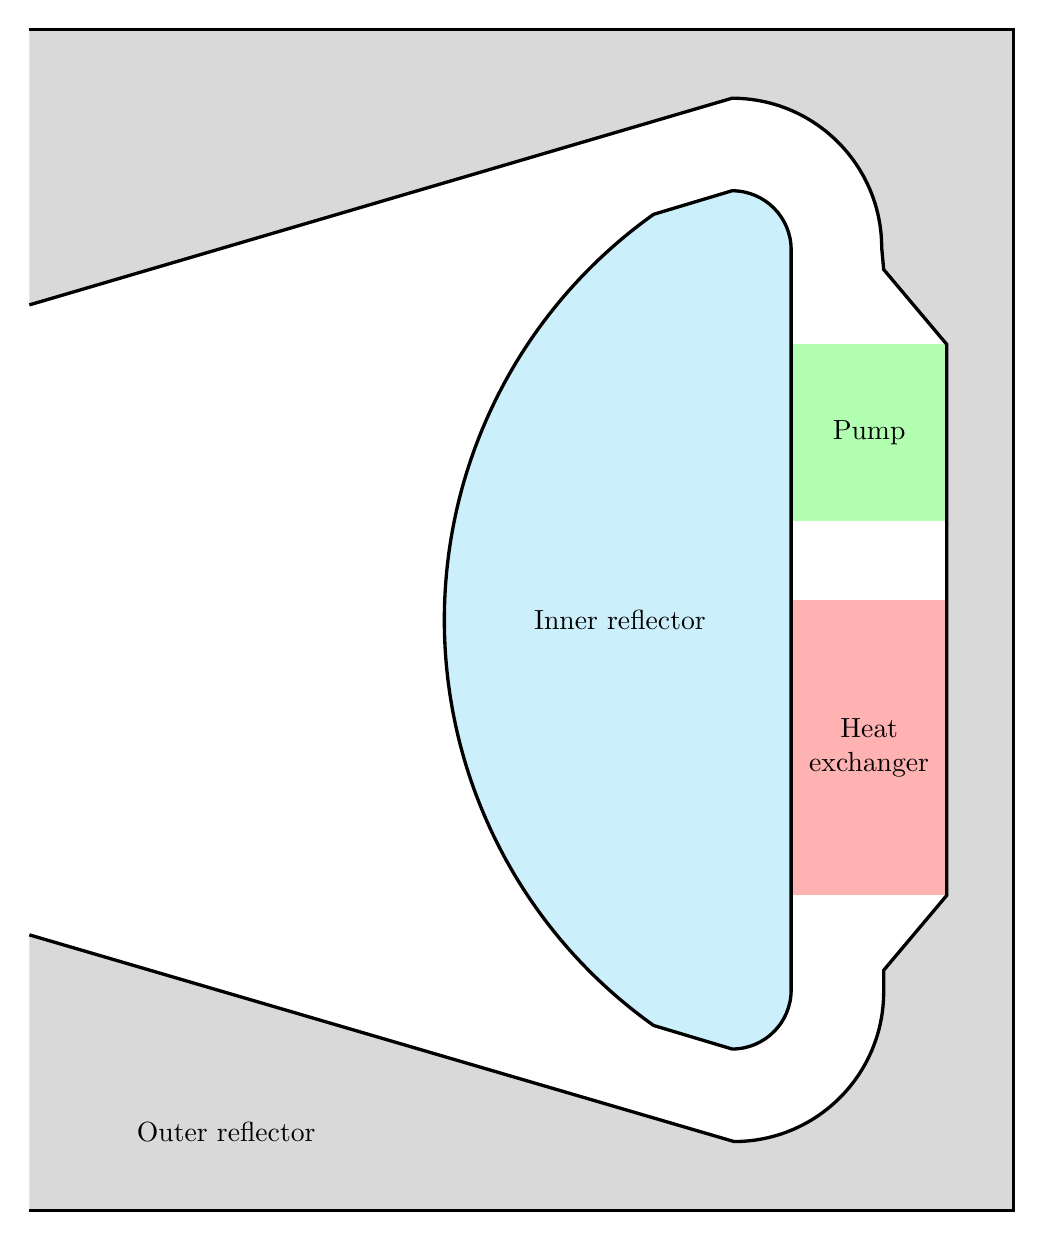
\begin{tikzpicture}
\begin{scope}[scale=5]
  % Shade the pump and heat exchanger regions.
  \fill[green!30!white] (1.935, 0.25) rectangle (2.33, 0.7);
  \fill[red!30!white] (1.935, -0.7) rectangle (2.33, 0.05);
  % Shade the outer reflector.
  \fill[black!15!white] (0, 0.8) -- (1.785, 1.325) arc (90:0:0.38)
    -- (2.17, 0.89) -- (2.33, 0.70) -- (2.33, -0.70) -- (2.17, -0.89)
    -- (2.17, -0.945) arc (0:-90:0.38) -- (0, -0.8) -- (0, -1.5) -- (2.5, -1.5)
    -- (2.5, 1.5) -- (0, 1.5) -- cycle;
  % Draw the boundaries of the fluid region.
  \draw[very thick] (0, 0.8) -- (1.785, 1.325) arc (90:0:0.38) -- (2.17, 0.89)
    -- (2.33, 0.70) -- (2.33, -0.70) -- (2.17, -0.89) -- (2.17, -0.945)
    arc (0:-90:0.38) -- (0, -0.8);
  \draw[very thick, fill=cyan!20!white] (1.5857, -1.0302) arc
    (234.59:125.41:1.264) -- (1.785, 1.09) arc (90:0:0.15) -- (1.935, -0.94)
    arc (0:-90:0.15) -- cycle;
  % Draw the vessel boundaries.
  \draw[very thick] (0, -1.5) -- (2.5, -1.5) -- (2.5, 1.5) -- (0, 1.5);
  % Annotate the pump and heat exchanger.
  \node at (2.133, 0.475) {Pump};
  \node[text width=16mm, align=center] at (2.133, -0.325) {Heat\\exchanger};
  % Annotate the reflectors.
  \node at (1.5, 0) {Inner reflector};
  \node at (0.5, -1.3) {Outer reflector};
\end{scope}
\end{tikzpicture}
\end{document}
